\documentclass[a4paper,oneside,11pt,DIV=12]{scrartcl}

\usepackage[utf8]{inputenc}
\usepackage{graphicx}

\setkomafont{captionlabel}{\sffamily\bfseries\small}
\setkomafont{caption}{\sffamily}

\usepackage[T1]{fontenc}
\usepackage{times}
\renewcommand{\familydefault}{\rmdefault} 

\usepackage{amssymb,amsmath,amsthm,mathrsfs}
\usepackage{bbm}
\usepackage{bm}
\usepackage[longnamesfirst]{natbib}
\usepackage{booktabs}
\usepackage{enumerate}
\usepackage{tikz}

\usepackage{setspace}
\setlength\parindent{24pt}

\newcommand{\code}[1]{{\texttt{#1}}}
\newcommand{\R}{{\mathbbmss R}} % Real Numbers

\usepackage{algorithmicx}
\usepackage{algpseudocode}

\usepackage{hyperref}
\hypersetup{
    colorlinks=true,
    linkcolor=blue,
    filecolor=blue,      
    urlcolor=blue,
    citecolor=blue
}

% ==============================================================================
\begin{document}
\shortcites{anderson_bai_etal_1999}
\shortcites{blackford_petitet_etal_2002}

\title{\Large Implementation Details on the Weighted BACON Algorithms}

\author{{\normalsize Tobias Schoch} \\ 
\begin{minipage}[t][][t]{\textwidth}
	\begin{center}
	\small{University of Applied Sciences Northwestern Switzerland FHNW} \\
	\small{School of Business, Riggenbachstrasse 16, CH-4600 Olten} \\
	\small{\texttt{tobias.schoch{@}fhnw.ch}}
	\end{center}
\end{minipage}} 

\date{{\small \today}}
\maketitle

\vspace{1em}
\hrule
\vspace{-0.5em}
\setcounter{tocdepth}{2}
\tableofcontents
\vspace{0.5em}
\hrule
\vspace{1em}

%------------------------------------------------------------------------------
\section{Introduction}\label{ch:introduction}
\setstretch{1.1}
Outlier detection and robust regression are computationally hard problems. This is all the more true when the number of variables and observations grow rapidly. Among all the candidate methods, the BACON algorithm (blocked adaptive computationally efficient outlier nominators) of \citet{billor_hadi_etal_2000} has favorable computational characteristics as it requires only a few model evaluation irrespective of the sample size. This makes it a superior algorithm for big data applications. 

In this document, we discuss the implementation of the BACON algorithm of \citet{billor_hadi_etal_2000} and some of its generalizations for multivariate outlier detection and robust linear regression.

%------------------------------------------------------------------------------
\subsection{Contribution and comparison with existing implementations} 
The BACON algorithms for multivariate outliers detection and robust linear regression are implemented in the \code{R} package \code{robustX} \citep{stahel_maechler_etal_2019}. The algorithms do not take the sampling weights into account. The multivariate outlier detection method of \citet{beguin_hulliger_2008} that is capable of dealing with sampling weights and missing values can be found in the \code{R} package \code{modi} \citep{hulliger_sterchi_2020}.

\begin{itemize}
	\item excesively copying
\end{itemize}
 

\begin{itemize}
	\item partial sort
	\item updating
	\item approximation chi 
\end{itemize}
 
The implementation of the BACON algorithms in the two mentioned packages is written in the \code{R} statistical software \citep{r-development-core-team_2020}.
The algorithms are implemented in the C language with an API for the R statistical software .



%------------------------------------------------------------------------------
\subsection{The BACON algorithms in a nutshell}\label{sec:nutshell} 
Suppose that the data at hand are $n$ observations on $p$ variables, $p < n$. The data are represented as the $(n \times p)$ matrix $\bm X = (\bm x_1, \ldots, \bm x_n)^T$ and are known to be contaminated by outliers. But it is not known which observations are outliers and how many observations are outliers.   

Let us fix some notation. Denote by $\mathscr{S}=\{1, \ldots, n\}$ the set of row indices of $\bm X$. Fix a set $S$ such that $S \subseteq \mathscr{S}$. We write $\bm X \vert_{S}$ to mean the row-wise restriction of $\bm X$ to the rows indexed by the elements of set $S$. For instance, let $S=\{1,3\}$; then $\bm X \vert_{S}$ is the $(2 \times p)$ matrix that consists of the rows 1 and 3 of $\bm X$. The complement of $S$ is denoted by $S^c$. The cardinality of a set $S$ is denoted by $\vert S \vert$. For ease of notation, we write $\bm X \vert_S^T$ instead of $(\bm X \vert_S)^T$ for the transpose of the restricted matrix. 

%------------------------------------------------------------------------------
\subsubsection{Multivariate outlier detection} 
Following \citet{billor_hadi_etal_2000}, the BACON multivariate outlier detection method consists of two algorithms (called Algorithm 2 and 3), which are applied to the data in series. 

\vspace{1em}
\noindent \textbf{\sffamily Algorithm 2.} The BACON algorithm is initialized by the computation of the center $\bm c$ of the data; see left panel in Fig. \ref{fig:schematic}; there, we have $\bm c = (c_1, c_2)^T$. In order to achieve good overall robustness, the center $\bm c$ is computed as the component-wise median \citep[][see Version 2 of Algorihm 2]{billor_hadi_etal_2000}. Next, the distances $d_i = \Vert \bm x_i - \bm c \Vert_2$ about the center are computed for all $i = 1,\ldots,n$, where $\Vert \cdot \Vert_2$ denotes the Euclidean norm. Then, we select the $m$ observations with the smallest $d_i$'s into the initial basic subset $S$, where $m = cp$ and $c$ is a tuning constant chosen by the user. 

\begin{figure}[htb]
	\centering
	\caption{Schematic illustration}\label{fig:schematic}	
	\vspace{1em}
	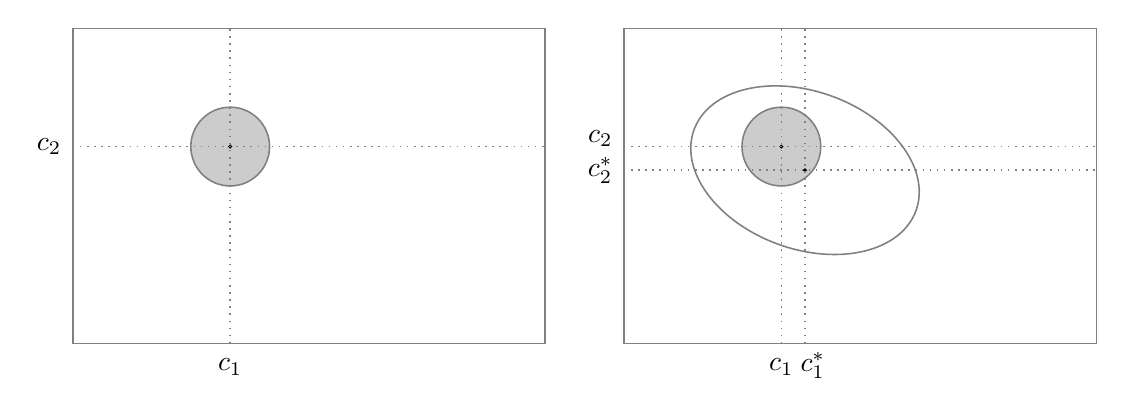
\begin{tikzpicture}[font = \sffamily, scale = 2]
		\def\myfontscale{1}
		\def\mylinewidth{0.2mm}
		%--------------------

		\draw[gray, line width = \mylinewidth] (0,0) rectangle (3,2);

		\filldraw[color=gray, fill=gray!40, line width = \mylinewidth](1,1.25) circle (0.25);
		\filldraw[black] (1,1.25) circle (0.25pt);

		\draw[dotted, gray, line width = \mylinewidth] (1,0) -- (1,2);
		\draw[dotted, gray, line width = \mylinewidth] (0, 1.25) -- (3, 1.25);
		\node[scale = \myfontscale] at (1, -0.15) {$c_1$};
		\node[scale = \myfontscale] at (-0.15, 1.25) {$c_2$};

		%--------------------
		\draw[gray, line width = \mylinewidth] (3.5,0) rectangle (6.5,2);

		\filldraw[color=gray, fill=gray!40, line width = \mylinewidth](4.5,1.25) circle (0.25);
		\filldraw[black] (4.5,1.25) circle (0.25pt);

		\draw[color=gray, shift = {(4.65, 1.1)}, rotate = 70, line width = \mylinewidth] (0, 0) ellipse (0.5 and 0.75);
		\filldraw[black] (4.65,1.1) circle (0.25pt);

		\draw[dotted, gray, line width = \mylinewidth] (4.5,0) -- (4.5,2);
		\draw[dotted, gray, line width = \mylinewidth] (3.5, 1.25) -- (6.5, 1.25);
		\node[scale = \myfontscale] at (4.5, -0.15) {$c_1$};
		\node[scale = \myfontscale] at (3.35, 1.3) {$c_2$};

		\draw[dotted, gray, line width = \mylinewidth] (4.65,0) -- (4.65,2);
		\draw[dotted, gray, line width = \mylinewidth] (3.5, 1.1) -- (6.5, 1.1);
		\node[scale = \myfontscale] at (4.7, -0.14) {$c_1^*$};
		\node[scale = \myfontscale] at (3.35, 1.1) {$c_2^*$};
    \end{tikzpicture}
\end{figure}

\noindent \textbf{\sffamily Algorithm 3.}  
\begin{enumerate}[Step 1)]
	\item For $\bm X\vert_S$, we compute
	%
	\begin{itemize}
		\item the component-wise arithmetic mean $\bm \mu_S$;
		\item the covariance/ scatter matrix $\bm \Sigma_S$. 
		\item If $\Sigma_S$ is singular, we keep adding observations to the subset $S$ until $\Sigma_S$ is nonsingular. Observations to be added are taken from the pool of the observations in the set $\mathscr{S} \setminus S$; in particular, we add those observations with the smallest $d_i$'s.
	\end{itemize}
	\item For all $i=1,\ldots,n$, compute the Mahalanobis distances
	\begin{equation}\label{eq:mahalanobis}
		d_i = \sqrt{(\bm x_i - \bm \mu_S)^T \bm \Sigma_S^{-1} (\bm x_i - \bm \mu_S)}
	\end{equation}
	and select all observations into the new subset $S^*$ (see right panel in Fig. \ref{fig:schematic}) whose $d_i$'s are smaller than the criterion $c_{np} \chi_{\alpha, p}^2$, where $\chi_{\alpha,p}^2$ is the $1-\alpha$ quantile of the chi-square distribution with $p$ degrees of freedom, and
	\begin{equation}\label{eq:criterion}
		c_{np} = 1 + \frac{p + 1}{n - p} + \frac{2}{n - 1 - 3p}.
	\end{equation}
	%
	\item If $S = S^*$ we terminate the updating scheme; otherwise, we let $S \gets S^*$ and jump to Step 1).
\end{enumerate}

\vspace{1em}
\noindent\textbf{\sffamily \small \itshape Remarks.}
\vspace{-0.5em}
\begin{enumerate}[i)]
	\item Upon termination, the set of outliers is given by $\mathscr{S} \setminus S^*$.
	%
	\item The above algorithm generates a sequence of subsets, say, $\{S_i : 0=1, \ldots\}$. The last subset in the sequence is the final subset of ``outlier-free'' observations. It is important to note that the subsets in the sequence are \textit{not  nested}; i.e., for any $i>0$, it is not guaranteed that $S_i \subset S_{i+1}$ (although eventually it will happen that $S_{i+1}$ is equal to $S_i$; hence, the algorithm terminates). 
	%
	\item The algorithm is initialized at the center $\bm c$, which is computed as the component-wise median (cf. Version 2 of Algorithm 2). As a consequence, the estimators of location and scatter are not affine equivariant; still, this proposal leads to nearly affine equivariant estimators \citep{billor_hadi_etal_2000}. By contrast, Version 1 of Algorithm 2 of \citet{billor_hadi_etal_2000} is affine equivariant by design as it takes the component-wise arithmetic mean as $\bm c$. But this choice has a considerably lower breakdown point.    
	%
	\item The breakdown point of Version 2 of the BACON algorithm has a breakdown point of approximately 40\% \citep{billor_hadi_etal_2000}.
	%
	\item \citet{beguin_hulliger_2008} generalized the BACON algorithms for outlier detection to account for sampling weights (survey data) and missing values. 
\end{enumerate}

%------------------------------------------------------------------------------
\subsubsection{Robust linear regression} 
Denote by $\bm X$ the $(n \times p)$ design matrix with full column rank $p$ ($p < n$). The response variable is written as the (column) $n$-vector $\bm y$. We want to compute the unknown parameter $\bm \beta \in \R^p$ in the overdetermined linear system 
\begin{equation*}
	\bm X \bm \beta = \bm y. 
\end{equation*}
\noindent In the presence of outliers in $\bm X$ \textit{and/or} $\bm y$, the least squares methods is (heavily) biased and/or inefficient as an estimator of the population regression parameter. Therefore, \citet{billor_hadi_etal_2000} proposed to search for a subset $S$ that is outlier-free and then to consider estimating $\bm \beta_S$, which solves the system 
\begin{equation}\label{eq:linsystem0}
	\bm X \vert_{S} \; \bm \beta_S = \bm y \vert_{S}. 
\end{equation}

Following \citet{billor_hadi_etal_2000}, the BACON robust linear regression method consists of algorithms (called Algorithm 4 and 5), which are applied to the data in series. 

\vspace{1em}
\noindent \textbf{\sffamily Algorithm 4.}  
\begin{enumerate}[Step 1)]
	\item Apply Algorithm 3 to the $\bm X$ data (having removed the column of $\bm X$ that contains the regression constant, if there is a constant) to obtain the subset $S$ of outlier-free observations. If $\mathrm{rank}(\bm X\vert_S) \neq p$, we keep adding observations to $S$ until $\bm X \vert_S$ is of full rank. The observations to be added are taken from the pool of the observations in the set $\mathscr{S} \setminus S$, whose Mahalanobis distances are smallest.
	%
	\item Solve (\ref{eq:linsystem0}) for $\bm \beta_S$, and compute the residual scale $\sigma_S = \Vert \bm r^T \bm r \Vert_2 / (\Vert S\Vert - p)$, where $\bm r = \bm y \vert_S - \bm X\vert_S \bm \beta_S$. Compute $\bm t_S=(t_1, \ldots, t_n)^T$, where
	\begin{equation}\label{eq:tis0}
		t_i = \begin{cases}
			\displaystyle{\frac{y_i - \bm x_i^T \bm \beta_S}{\sigma_S \sqrt{1 - \bm x_i^T (\bm X^T \vert_S \bm X \vert_S)^{-1}\bm x_i}}} & \text{if} \; i \in S,\\
			\displaystyle{\frac{y_i + \bm x_i^T \bm \beta_S}{\sigma_S \sqrt{1 - \bm x_i^T (\bm X^T \vert_S \bm X \vert_S)^{-1}\bm x_i}}} & \text{otherwise}.
		\end{cases}
	\end{equation}
	%
	\item Let $k \gets p + 1$ 
	\item Select the $k$ observations whose $t_i$'s are smallest (in absolute value) into the subset $S$. If $\mathrm{rank}(\bm X \vert_S)\neq p$, we keep adding observations from $\mathscr{S} \setminus S$ (with the smallest $t_i$'s) to $S$ until $\bm X \vert_S$ is of full rank. The set $S$ is called the initial basic subset.
	%
	\item If $k \leq m$, let $k \gets k + 1$ and go to Step 4); otherwise terminate. 
\end{enumerate}

Algorithm 4 generates a sequence of subsets, say, $\{S_i : 0=1, \ldots\}$. It is important to note that the subsets in the sequence are \textit{not} nested.

\vspace{1em}
\noindent \textbf{\sffamily Algorithm 5.}  
\begin{enumerate}[Step 1)]
	\item Use Algorithm 4 to select a subset $S_0$ of size $m = c\cdot p$, where the constant $c$ can be chosen by the user; \citet{billor_hadi_etal_2000} recommend a value of 4 or 5.
	\item For $S_0$, compute the $t_i$'s in (\ref{eq:tis0}) and select a new subset, say, $S_1$ that consists of all observations whose $t_i$'s are (in absolute value) smaller than the $\alpha/2(\vert S_1 \vert +1)$ quantile of the Student $t$-distribution with $\vert S_1 \vert - p$ degrees of freedom.
	\item If $S_0 \neq S_1$, let $S_1 \gets S_0$ and go to Step 2); otherwise terminate.
\end{enumerate}

\vspace{1em}
\noindent\textbf{\sffamily \small \itshape Remark.} Upon termination, Algorithm 5 provides the robust estimate $\bm \beta_S$ of the population regression parameter $\bm \beta$ and the regression scale estimate $\sigma_S$. 

%------------------------------------------------------------------------------
\section{Weighted BACON algorithm}
%------------------
\subsection{Location and scatter}
Let $S \subseteq \mathscr{S}$. We denote the weighted column means of $\bm X \vert_S$ (Hajek estimator) by
 \begin{equation}\label{eq:weightedmean}
 	\bm \mu_S = \frac{1}{W_S}\sum_{i \in S} w_i \bm x_i, \qquad \text{where} \quad W_S = \sum_{i \in S} w_i,
 \end{equation}
\noindent and define the matrix $\bm Z_S$ (which is equal to $\bm X\vert_S$ centered or shifted by $\bm \mu_S$ and appropriately scaled)
\begin{equation}\label{eq:x_centered_scaled}
	\bm Z_S = \sqrt{\frac{\bm w\vert_S}{W_S - 1}} \circ \big( \bm X\vert_S - \bm 1 \bm c_S^T \big),
\end{equation}
\noindent where $\bm 1$ is the vector of ones (of size $\vert S \vert$), $\circ$ denotes the Hadamard product, and $\sqrt{\cdot}$ is applied element by element. Note that the Gramian matrix $\bm Z_S^T \bm Z_S$ is equal to the scatter/ covariance matrix 
\begin{equation}\label{eq:weightedsigma}
	\bm Z_S \bm Z_S^T = \frac{1}{W_S - 1}\sum_{i \in S} w_i (\bm x_i - \bm \mu_S)(\bm x_i - \bm \mu_S)^T =:	\bm \Sigma_S.
\end{equation}

%------------------
\subsection{Mahalanobis distance}
The scatter matrix $\bm \Sigma_S$ is required to be nonsingular, for otherwise we cannot compute the Mahalanobis distances in (\ref{eq:mahalanobis}). There are several ways to check whether $\bm \Sigma_S$ is nonsingular. We prefer a method that is computationally cheap for the following reason: If $\bm \Sigma_S$ appears to be singular, we stop the computations on the current subset. Then, we keep adding observations to the set $S$ until $\bm \Sigma_S$ is nonsingular. Because the computational costs associated with growing the set $S$ are so small, it is not economical putting too much effort into a sophisticated method to check whether the scatter matrix is singular. 

We adopt a two-stage approach.
\begin{enumerate}[(1)]
	\item First, we count the number of positive elements on the diagonal of $\bm \Sigma_S$ (in floating-point arithmetic terms),
	 \begin{equation}\label{eq:nonsingular1}
		\widehat{r}_{\mathrm{pd}} = \sum_{i=1}^p \mathbbm{1} \big\{ (s_{ii}) > \epsilon \big\}, \qquad (s_{ij}) \equiv \Sigma_S,
	 \end{equation}
	where $\mathbbm{1}\{ \cdot \}$ is the indicator function, and $\epsilon$ is the machine epsilon (double precision). If $\widehat{r}_{\mathrm{pd}} \neq p$, the computations are stopped and we switch to the process of enlarging the subset $S$ until $\widehat{r} = p$.

	This approach is very effective as it catches the most common case of nonsingularity (non positive-definiteness) while its computational costs are negligible. To see this, suppose a subset $S$ such that one column (variable) of $\bm X\vert_S$ is constant; hence, the variance is zero (e.g. grouped data).
	%
	\item In the second step, we compute the factorization 
	\begin{equation}\label{eq:chol}
		\bm \Sigma_S = \bm L_S \bm L_S^T. 
	\end{equation}
	If $\bm \Sigma_S$ is positive definite, the factorization in (\ref{eq:chol}) is the (unique) Cholesky decomposition, where $\bm L$ is a lower triangular matrix with positive diagonal elements. If, however, $\bm \Sigma_S$ is positive \textit{semi}-definite it still has a decomposition of this form but the diagonal elements of $\bm L$ can be zero; see e.g. \citep[][Chap. 4.2.8]{golub_loan_1996}. Now, our approach is the following. 
	\begin{enumerate}[a)]
		\item  We compute the Cholesky decomposition in (\ref{eq:chol}) using the \code{LAPACK}: \code{dpotrf} subroutine \citep{anderson_bai_etal_1999}. 
		%
		\item If $\bm \Sigma_S$ is indeed positive semi-definite, the Cholesky decomposition can (or will) break down because a zero (or negative) pivot is encountered at some stage of the factorization. The subroutine \code{dpotrf} has an error flag (see argument \code{INFO}) that indicates when the factorization could not be completed because a leading minor of the matrix is not positive definite. If this flag has been raised, $\bm \Sigma_S$ is regarded as singular and we switch to the process of enlarging the subset $S$ until $\bm \Sigma_S$ is nonsingular.    
		%
		\item Relying on the error flag of \code{dpotrf} alone is too optimistic. Therefore, we also compute an estimate of the number of positive diagonal elements of $\bm L_S$,  
		\begin{equation}\label{eq:numericrank}
			\widehat{r} = \sum_{i=1}^p \mathbbm{1} \big\{ \bm (l_{ii}) > \delta \big\}, \qquad (l_{ii}) \equiv \bm L_S,
		\end{equation}
		\noindent where $\delta$ is a numerical constant. We pick a rather conservative choice for $\delta$, e.g., $\delta = \epsilon^{1/4}$, where $\epsilon$ is the machine epsilon (double precision). If $\widehat{r}\neq p$, $\bm \Sigma_S$ is regarded as singular and we switch to the process of enlarging the subset $S$ until $\bm \Sigma_S$ is nonsingular.  
	\end{enumerate}
\end{enumerate}

\vspace{1em}
\noindent\textbf{\sffamily \small \itshape Remarks.}
\vspace{-0.5em}
\begin{enumerate}[i)]
	\item Our two-stage approach is not ``fully waterproof'' but it is computationally inexpensive. 
	%
	\item In place of the two-stage approach, we could determine the numerical rank of $\bm Z_S$ by the singular value decomposition (SVD). That is, the numerical rank $\widehat{r}$ is computed as the largest integer in ($0, \ldots, p$) for which $\sigma_r \geq n\delta \sigma_1$, where $\delta$ is a tolerance criterion (e.g. $\delta = 1 \cdot 10^{-16}$) and $\sigma_1 \geq \cdots \geq \sigma_p$ are the singular values \citep[][Chap. 2.5.5]{golub_loan_1996}. Alternatively, we could use a rank-revealing Cholesky factorization with complete column pivoting \citep[\code{LAPACK:} \code{dpstrf},][]{anderson_bai_etal_1999} of $\bm \Sigma_S$ to determine its numerical rank. However, both approaches are computationally quite expensive. Another approach would be to check whether $\bm \Sigma_S$ is positive definite by checking if all of its eigenvalues of are positive (in exact arithmetic). In floating-point arithmetic, we compute the eigenvalues \citep[\code{LAPACK}: \code{dsyev},][]{anderson_bai_etal_1999} and then proceed as in the SVD-based. However, this approach is computationally still quite expensive.
\end{enumerate}

\noindent If $\bm \Sigma_S$ is nonsingular, we solve the triangular system of linear equations
\begin{equation}\label{eq:inverse_chol}
	\bm L_S \bm  A_S= \bm Z_S
\end{equation}
\noindent for the $(n \times p$) matrix $\bm A_S$ by forward substitution \citep[\code{BLAS}: \code{dtrsm},][]{blackford_petitet_etal_2002}, where $\bm L_S$ and $\bm Z_S$ are defined in, respectively, (\ref{eq:chol}) and  (\ref{eq:x_centered_scaled}). Mahalanobis distances in (\ref{eq:mahalanobis}) can now be computed (for all $i=1,\ldots, n$) by
\begin{equation}\label{eq:maha_chol}
	d_i = \sqrt{\sum_{j=1}^p (a_{ij}^2)}, \qquad (a_{ij}) \equiv \bm A_S. 
\end{equation}

%------------------------------------------------------------------------------
\subsection{Algorithms}
The following display shows pseudo-code of Algorithm 2 of \citet{billor_hadi_etal_2000}.  

\vspace{1em}
\noindent \textbf{\sffamily Algorithm 2.}  
\begin{algorithmic}[1]\label{}
	\setstretch{1.3}
	\hypertarget{alg:alg2}{\Require $\bm X$, $\bm w$, $m$}
	\State $\bm \zeta \gets$ \textsc{weighted\_median}$(\bm X, \bm w)$
	\Comment{component-wise weighted median}  
	\State $\bm d \gets (d_1, \ldots, d_n)$, where $d_i = \Vert \bm x_i - \bm \zeta \Vert_2$
	\State $S \gets$ \textsc{select\_subset}$(\bm d, m)$
	\Comment{select the set with the $m$ smallest $d_i$'s}
	\While {$m < n$}
		\State $\bm \mu_S \gets$ \textsc{weighted\_mean}$(\bm X\vert_S, \bm w\vert_S)$
		\Comment{Eq. (\ref{eq:weightedmean})}
		\State $\bm \Sigma_S \gets$ \textsc{weighted\_scatter}($\bm X\vert_S, \bm w\vert_S, \bm \mu_S)$
		\Comment{Eqs. (\ref{eq:x_centered_scaled}) and (\ref{eq:weightedsigma})}
		\If {$\widehat{r}_{\mathrm{pd}} = p$}
		\Comment{Eq. (\ref{eq:nonsingular1})}
			\State $\bm L_S \gets$ \textsc{cholesky\_decomposition}$(\bm \Sigma_S)$
			\Comment{Eq. (\ref{eq:chol})}
			\If {$\widehat{r} = p$}
				\Comment{Eq. (\ref{eq:numericrank})}
				\State \textbf{break}
			\EndIf
		\EndIf 
			\State $m \gets m + 1$
			\Comment{add obs. to the subset}
			\State $S \gets S \, \cup$ \textsc{index}$\big(\bm d[m]\big)$
			\Comment{\textsc{index} returns the indices}
	\EndWhile
	\State \Return $S$, $m$
	\Comment{return initial basic subset and its size}
\end{algorithmic}

\vspace{1em}
\noindent\textbf{\sffamily \small \itshape Remarks.}
\vspace{-0.5em}
\begin{enumerate}[i)]
	\item \textsc{weighted\_median}$(\bm X, \bm w)$ computes the weighted median for each column of $\bm X$. The weighted median is implemented as a weighted quickselect algorithm; see Section \ref{sec:utility}. 
	\item \textsc{select\_subset}$(\bm d, m)$ partially sorts the elements of $\bm d$ such that the first $m$ elements are in their final (sorted) position. The indices of the first $m$ elements are selected into the subset, which is returned; see Section \ref{sec:utility} for more details.
	\item In the \code{while} loop, we keep adding observations to the subset until the scatter matrix $\bm \Sigma_S$ is nonsingular.
\end{enumerate}

\vspace{1em}
\noindent The following display shows pseudo-code of Algorithm 3 of \citet{billor_hadi_etal_2000}.

\vspace{1em}
\noindent \textbf{\sffamily Algorithm 3.}  
\begin{algorithmic}[1]
	\setstretch{1.3}
	\hypertarget{alg:alg3}{\Require $\bm X$, $\bm w$, $S$, $m$} from \hyperlink{alg:alg2}{\textsc{algorithm} 2}
	\Comment{initial basic subset and its size}
	\State $S_1 \gets \{\}$
	\Comment{initialize $S_1$ as the empty set}
	\While {$m < n$}
		\State $\bm \mu_S \gets$ \textsc{weighteed\_mean}$(\bm X\vert_S,\, \bm w\vert_S)$
		\Comment{Eq. (\ref{eq:weightedmean})}
		\State $\bm \Sigma_S \gets$ \textsc{weighted\_scatter}$(\bm X\vert_S, \, \bm w\vert_S)$
		\Comment{Eqs. (\ref{eq:x_centered_scaled}) and (\ref{eq:weightedsigma})}
		\State $\bm L_S \gets$ \textsc{cholesky\_decomposition}$(\bm \Sigma_S)$
		\Comment{Eq. (\ref{eq:chol})}
		\State $\bm d_S = (d_1, \ldots, d_n)^T  \gets$ \textsc{mahalanobis\_distance}$\big(\bm X, \bm L, S \big)$
		\State $S_1 \gets$ \textsc{index}$\big( \bm d_S < c_{np}\cdot \chi_{p,\alpha}^2\big)$
		\Comment{new subset}
		\State $m \gets \vert S_1\vert$
		\If {$S = S_1$}
			\State \textbf{break}
		\EndIf
		\State $S \gets S_1$
	\EndWhile
	\State \Return $\mu_S$, $\Sigma_S$, $S$, $m$
\end{algorithmic}

\vspace{1em}
\noindent\textbf{\sffamily \small \itshape Remarks.}
\vspace{-0.5em}
\begin{enumerate}[i)]
	\item The return values of Algorithm 3 are the final subset $S$, its size $m$, the weighted mean $\bm \mu$, and the weighted scatter/covariance matrix $\bm \Sigma_S$ on the subset $S$. 
	%
	\item The function \text{mahalanobis\_distance} at Line 6 computes the Mahalanobis distances for all $i \in \mathscr{S}$; it solves (\ref{eq:inverse_chol}) and then computes the $d_i$'s defined in  (\ref{eq:maha_chol}).
	%
	\item The chi-square criterion $c_{np}\cdot \chi_{p,\alpha}^2$ at Line 7 is defined in (\ref{eq:criterion}).
\end{enumerate}	


%------------------------------------------------------------------------------
\section{Weighted BACON regression algorithm}
Denote by $\bm X$ the $(n \times p)$ design matrix with full column rank $p$ ($p < n$). The response variable is written as the (column) $n$-vector $\bm y$. Fix $S$ such that $S \subseteq \mathscr{S}$, $\vert S \vert \geq p$, and consider the least squares (LS) estimator $\bm \beta_S \in \R^p$ which solves the normal equations 
\begin{equation}\label{eq:leastsquares}
	\bm X \vert_{S}^T \; \bm X \vert_{S} \; \bm \beta_S =  \bm X \vert_S^T \;\bm y \vert_{S}. 
\end{equation}

\textbf{\sffamily Note.} The weighted least squares estimator obtains by replacing $\widetilde{\bm X} \vert_S$ and $\widetilde{\bm y} \vert_S$ with, respectively, $\widetilde{\bm X}\vert_S = (\sqrt{\bm w} \circ \bm X)\vert_S$ and $\widetilde{\bm y}\vert_S = (\sqrt{\bm w} \circ \bm y)\vert_S$, where $\sqrt{\cdot}$ is applied element by element, and $\circ$ denotes the Hadamard product.  

The solution of the normal equations in (\ref{eq:leastsquares}) is known to be numerically unstable \citep[][Chap. 5.3]{golub_loan_1996}. Therefore, we consider solving the LS problem by the QR factorization, which is stable but computationally rather expensive. Suppose that $\bm X\vert_S$ has full column rank. Define the ``thin'' QR factorization of $\bm X \vert_{S}$ \citep[][Chap. 5.3]{golub_loan_1996} 
\begin{equation}\label{eq:reg_qr1}
	\bm X \vert_S = \bm Q \bm R =  \big( \bm Q_{S}^1, \; \bm Q_{S}^2 \big) \left(\begin{matrix} \bm R_{S}^1 \\ \bm 0_S \end{matrix}\right) = \bm Q_{S}^1 \bm R_{S}^1,
\end{equation}
\noindent where $\bm R_{S}^1$ is an $(p \times p)$ upper triangular matrix and $\bm Q_{S}^1$ is an $(\vert S \vert \times p)$ orthogonal matrix; the matrices $\bm 0_{S}$ and $\bm Q_{S}^2$ are of conformable size but of no further interest. The parameter $\bm \beta_S$ solves the triangular system   
\begin{equation}
	\bm R_{S}^1 \, \bm \beta_S  = (\bm Q_{S}^1)^T \, \bm y \vert_S.
\end{equation}

A key characteristic of the BACON algorithm for regression is that the subset $S$ is enlarged over several steps. To see this, let the design matrix $\bm X$ be of dimension $n=1\,000$ with $p=4$ variables. In the first step (see Section \ref{sec:nutshell}), \hyperlink{alg:alg3}{Algorithm 3} is called on $\bm X$. We suppose that the resulting initial subset is of size 700. In step 2, we apply \hyperlink{alg:alg4}{Algorithm 4} to select $k \gets p+1$ observations with the smallest distances. Then, we keep growing $k \gets k + 1$ as long as $k \leq m$, where $m=cp$ and $c$ is typically chosen to be 4 or 5. Let's take $c=5$. Then, we observe the following sequence of subset sizes  
\begin{verbatim}
    700, 5, 6, 7, 8, 9, 10, 11, 12, 13, 14, 15, 16, 17, 18, 19, 20 
\end{verbatim}
\noindent until we can start with Algorithm 5. The computation of the QR factorization for each instance along this sequence is computationally quite expensive. Fortunately, an updating scheme for the QR factorization is available such that we do not have to re-compute the entire factorization over and over. The computational costs of the updating scheme are far less than recomputing the decomposition.

%--------------------------------------
\subsection{Up- and dating schemes}
We consider up- and downdating separately.

%--------------------------------------
\subsubsection{Updating}

Consider the subset $S$ and the QR factorization of $\bm X \vert_S$ in (\ref{eq:reg_qr1}) $\bm X \vert_S = \bm Q_S^1 \bm R_S^1$. Suppose that the subset $S$ is enlarged by one element. To be specific, we shall assume that the $k$th element is added to the subset; hence, $S_{+} = S \cup \{k\}$. The design matrix associated with the enlarged subset obtains by appending the $k$th row of $\bm X$ to $\bm X \vert_S$, 
\begin{equation*}
	\bm X\vert_{S_+} = \left[\begin{matrix}
		\bm X\vert_{S} \\ \bm x_k^T 
	\end{matrix}\right].
\end{equation*}
\noindent Let $\bm G_1, \ldots, \bm G_p$ denote Givens rotation matrices (i.e., planar rotation matrices); see e.g. \citet[][Chap. 5.1.8]{golub_loan_1996}. Premultiplication by a Givens rotation matrix amounts to a counterclockwise rotation (given some rotation angle). In particular, the rotation matrices can be determined such that
\begin{equation}\label{eq:reg_qr2}
	\bm G_1^T \cdots \bm G_p^T \bm H = \bm R_{S}^1
\end{equation}
\noindent is a upper triangular matrix; $\bm H$ is an upper Hessenberg matrix. It then follows that \citep[][Chap. 12.5.3]{golub_loan_1996} the QR factorization of $\bm X\vert_{S_+}$ is $\bm X\vert_{S_+} = \bm Q_{S_+}^1 \bm R_{S_+}^1$, where 
\begin{equation}\label{eq:reg_qr3}
	\bm Q_{S_+}^1 = \mathrm{diag}\big(1, \bm Q_{S}^1\big) \bm G_1 \cdots \bm G_p.
\end{equation}
\noindent In other words, the identities (\ref{eq:reg_qr2}) and (\ref{eq:reg_qr3}) describe a scheme for updating the matrices $\bm R_S^1$ and $\bm Q_S^1$ to get $\bm R_{S_+}^1$ and $\bm Q_{S_+}^1$. There exists a similar method to downdate the QR factorization (i.e., removing a row from $\bm X \vert_S$). The downdating scheme is more intricate as it can break down when the matrix becomes indefinite. We shall discuss this later.  

Updating $\bm R_S^1$ is straightforward and inexpensive (order $p^2/2$ flops). In contrast, updating $\bm Q_S^1$ is more expensive (order $n^2$ flops). Therefore, we take a different approach. Our approach is based on the observation that $\bm R_S^1 = \bm L_S^T$, where $\bm L_S$ is a lower triangular matrix, i.e. the Cholesky factor of the Gramian matrix $\bm X\vert_S^T \bm X \vert_S$. So, we initialize the regression estimator by the QR factorization, and then we switch to a Cholesky-based regression approach,  
\begin{equation}
	\bm L_S \, \bm L_S^T \, \bm \beta_S = \bm X\vert_S^T \, \bm y\vert_S \qquad \Longleftrightarrow \qquad \bm L_S \, \bm u_S = \bm X\vert_S^T \, \bm y\vert_S, 
\end{equation}
\noindent where $\bm u_S = \bm L_S^T \, \bm \beta_S$. For the Cholesky-based approach, we solve 
\begin{equation}\label{eq:chol_reg}
	\bm \beta_S \gets \text{\textsc{forward\_solve}}\Big(\bm L_S, \; \text{\textsc{forward\_solve}}\big(\bm L_S, \bm (X^T \bm y)\vert_S\big)\Big).
\end{equation}
\noindent The Cholesky regression aproach is computationally less expensive than the QR aproach. Its flop counts is of order $p^2(n + p/3)$, whereas the QR algorithm requires $2p^2(n-p/3)$ flops; see e.g. \citet[][Chap. 5.3]{golub_loan_1996}.

For the Cholesky-based approach, the updating scheme is as follows (let $S_{+} = S \cup \{k\}$). First, we compute, the rank-one update of $\bm X\vert_S^T \, \bm y\vert_S$,
\begin{equation}\label{eq:xtyupdate}
	\bm X\vert_{S_+}^T \, \bm y_{S_+} = \bm X\vert_{S}^T \, \bm y \vert_S + y_k \bm x_k^T.
\end{equation}
\noindent Second, the Cholesky factor $\bm L_S$ is updated by the following function \citep[][p. 340]{stewart_1998}. 
\begin{algorithmic}[1]
	\setstretch{1.3}
	\hypertarget{alg:cholupdate}{\Function{chol\_update}{}$(\bm L, \bm x)$}
	\For{$i=1,\ldots,p$}
		\State  \hyperlink{alg:setuprotation}{\textsc{setup\_rotation}}$\big(\bm L_S[i,i], \bm x[i], c, s\big)$
		\State \hyperlink{alg:applyrotation}{\textsc{apply\_rotation}}$\big(\bm L_S[i, i+1:p], \bm x[i+1:p], c, s\big)$
	\EndFor
	\EndFunction 
\end{algorithmic}
\noindent where $\bm L_S[i,j]$ denotes the $i$th row and $j$th column of $\bm L_S$. The functions \hyperlink{alg:setuprotation}{\textsc{setup\_rotation}} and \hyperlink{alg:applyrotation}{\textsc{apply\_rotation}} are defined as follows \citep[][Algorithms 1.6 and 1.7]{stewart_1998}.
\begin{algorithmic}[1]
	\setstretch{1.3}
	\hypertarget{alg:setuprotation}{\Function{setup\_rotation}{}$(a,b,c,s)$}
	\State $\tau \gets \vert a \vert + \vert b \vert$
	\If{$\tau \leq \epsilon$}
		\State $c \gets 1$; $\quad s \gets 0$
		\State \Return
	\EndIf
	\State $\nu \gets \tau \sqrt{(a/\tau)^2 + (b/\tau)^2}$
	\State $c \gets a/\nu$; $\quad s \gets b/\nu$
	\State $a \gets \nu$; $\quad b \gets 0$
	\EndFunction
\end{algorithmic}
\begin{algorithmic}[1]
	\setstretch{1.3}
	\hypertarget{alg:applyrotation}{\Function{apply\_rotation}{}$(c, s, \bm x, \bm y)$}
	\State $\bm t \gets c \bm x + s \bm y$
	\State $\bm y \gets c \bm y - s \bm x$
	\State $\bm x \gets \bm t$
	\EndFunction
\end{algorithmic}

\vspace{1em}
\noindent\textbf{\sffamily \small \itshape Remarks.}
\vspace{-0.5em}
\begin{enumerate}[i)]
	\item The scaling factor $\tau$ in function \hyperlink{alg:setuprotation}{\textsc{setup\_rotation}} is introduced to avoid overflows and make underflows harmless; see \citet[][p. 273]{stewart_1998} and \citet[][Chap. 5.1.8]{golub_loan_1996}. 
	%
	\item The \code{C} library \code{math.h} provides (since standard \code{C99}) the dedicated function \code{hypot(x,y)} for the computation of $\sqrt{x^2 + y^2}$ (see Line 7 of  \hyperlink{alg:setuprotation}{\textsc{setup\_rotation}}) without undue overflow or underflow at intermediate stages of the computation.
	%
	\item The complexity of function \hyperlink{alg:cholupdate}{\textsc{chol\_update}} is of order $p^2/2$ flops \citep[][p. 340]{stewart_1998}. 
\end{enumerate}

%--------------------------------------
\subsubsection{Downdating scheme}
The downdating scheme is more intricate as it can break down when the matrix becomes indefinite. Let $S_{-} = S \setminus \{k\}$. The rank-one downdate of $\bm X\vert_S^T \, \bm y\vert_S$ is unproblematic and is given by
\begin{equation}\label{eq:xtydowndate}
 	\bm X\vert_{S_-}^T \, \bm y_{S_-} = \bm X\vert_{S}^T \, \bm y \vert_S - y_k \bm x_k^T. 
\end{equation}

There exist three algorithms for downdating the Cholesky factor $\bm L$ \citep[][p. 355]{stewart_1998}: Saunder`s method, the methods of mixed rotation, and the methods of hyperbolic rotations. We use the method of mixed rotations, an implementation of which is the following algorithm \citep[][Algorithm 3.9]{stewart_1998}
\begin{algorithmic}[1]
	\setstretch{1.3}
	\hypertarget{alg:choldowndate}{\Function{chol\_downdate}{}$(\bm L, \bm x)$}
	\For{$i=1,\ldots,p$}
		\State $a \gets \bm L[i,i]^2 - \bm x[i]^2$
		\If{$a < \epsilon$}
			\State \Return Error 
		\Else
			\State $b \gets \sqrt{a}$
		\EndIf
		\State $c \gets b/\bm L[i,i]$
		\State $s \gets \bm x[i] / \bm L[i,i]$
		\State $\bm L[i,i] \gets b$
		\State $\bm L[i, i+1:p] \gets \big( \bm L[i, i+1:p] - s \bm x[i+1:p]\big) / c$
		\State $\bm x[i+1:p] \gets c \bm x[i+1:p] - s \bm L[i, i+1:p]$
	\EndFor
	\EndFunction
\end{algorithmic}

\vspace{1em}
\noindent\textbf{\sffamily \small \itshape Remarks.}
\vspace{-0.5em}
\begin{enumerate}
	\item The constant $\epsilon$ (see Line 5) is taken to be the machine double epsilon. 
	%
	\item The function  \hyperlink{alg:choldowndate}{\textsc{chol\_downdate}} returns an \textsc{error} if downdating is not feasible (see line 5). This happens when the matrix $\bm L^T \bm L - \bm x \bm x^T$ associated with downdating is not positive definite. 
	%
	\item It might be thought that the appearance of a small $c$ leads to numerical instability. But this is not the case as \citet[][p. 346]{stewart_1998} shows, unless the problem is itself ill-conditioned. 
	%
	\item \citet[][p. 352]{stewart_1998} shows that the downdating scheme used in  \hyperlink{alg:choldowndate}{\textsc{chol\_downdate}} has some nice numerical properties; in particular, it is relationally stable (whereas the method of hyperbolic rotations is not).
	%
	\item The order of flops count of the functions \hyperlink{alg:choldowndate}{\textsc{chol\_downdate}} and \hyperlink{alg:cholupdate}{\textsc{chol\_update}} is the same \citep[][p. 346]{stewart_1998}. 
\end{enumerate}

%--------------------------------------
\subsubsection{Application of the up- and downdating schemes}
The functions \hyperlink{alg:cholupdate}{\textsc{chol\_update}} and \hyperlink{alg:choldowndate}{\textsc{chol\_downdate}} compute an update of the Cholesky factor when one row of the design matrix is added or removed. Let $S_0$ and $S_1$ be subsets. The following function takes care of all up-/ and downdates that result when we transition from set $S_0$ to set $S_1$. It returns up-/downdates of $\bm L_S$ and $\bm X^T_S\bm y_S$. 

\begin{algorithmic}[1]
	\setstretch{1.3}
	\hypertarget{alg:update}{\Function{update}{}}$\big(\bm L_{S_0}, \bm X, \bm y, S_0, S_1\big)$
		\State $U \gets S_0 \setminus S_1 \neq \{\}$
		\Comment{identify updates}
		\State $D \gets S_1 \setminus S_0 \neq \{\}$
		\Comment{identify downdates}
		\For{$u \in U$}
			\State $\bm L_{S_1} \gets$ \hyperlink{alg:cholupdate}{\textsc{chol\_update}}$\big( \bm L_{S_0}, \bm X \vert_{S_0 \setminus S_1}\big)$
			\State $(\bm X^T  \bm y)\vert_{S_1} \gets (\bm X^T \bm y)\vert_{S_0} + (\bm X^T \bm y)\vert_{S_0 \setminus S_1}$
			\Comment{see (\ref{eq:xtyupdate})}
		\EndFor

		\For{$u \in U$}
			\State $\bm L_{S_1} \gets$ \hyperlink{alg:choldowndate}{\textsc{chol\_downdate}}$\big( \bm L_{S_0}, \bm X \vert_{S_1 \setminus S_0}\big)$
			\Comment{returns \textsc{error} if downdating breaks}
			\If{\textsc{error}}
				\State \Return \textsc{error}
			\EndIf
			\State $(\bm X^T  \bm y)\vert_{S_1} \gets (\bm X^T \bm y)\vert_{S_0} - (\bm X^T \bm y)\vert_{S_1 \setminus S_0}$
			\Comment{see (\ref{eq:xtydowndate})}
		\EndFor
		\State \Return $\bm L_{S_1}, \;(\bm X^T  \bm y)\vert_{S_1}$
	\EndFunction
\end{algorithmic}

\vspace{1em}
\noindent\textbf{\sffamily \small \itshape Remark.} The ``mechanics'' underlying the function \hyperlink{alg:update}{\textsc{update}} are trivial. But it is important that the updates are computed in the first place, followed by the downdates. Otherwise we would experience too many breakdowns of the downdating algorithm.    

%--------------------------------------
\subsection{Residuals, ``hat'' matrix, and $t_i$'s}
Define the residuals
\begin{equation}\label{eq:residuals}
	\bm r(\bm \beta_S) = \big( r_1(\bm \beta_S), \ldots, r_n(\bm \beta_S) \big)^T = \bm y - \bm X \bm \beta_S
\end{equation}
\noindent for all $i = 1, \ldots, n$ and let 
\begin{equation}\label{eq:sigma}
	\sigma_S = \frac{ \big\Vert \; \bm r \vert_S \big(\bm \beta_S) \; \big\Vert_2}{\sqrt{\vert S \vert - p}} 
\end{equation}
\noindent denote the estimate of the residual scale (on the restriction). For the weighted regression, we have  
\begin{equation}
	\sigma_S = \frac{ \big\Vert \; \widetilde{\bm r} \vert_S \big(\bm \beta_S) \, \big \Vert_2}{\sqrt{ \sum_{i \in S} w_i - p}}, 
\end{equation}
\noindent where $\widetilde{\bm r}(\bm \beta_S) = \widetilde{\bm y} - \widetilde{\bm X} \bm \beta_S$.

The ``hat'' matrix of the LS estimate in (\ref{eq:leastsquares}), i.e., the orthogonal projection matrix onto the column space of $\bm X \vert_S$, is given by $\bm H_S = \bm Q_{S1} \, \bm Q_{S1}^T$. The diagonal elements of $\bm H_S$ are called leverages. The \textit{extension} of the projection matrix onto column space of the entire matrix $\bm X$ is given by 
\begin{equation*}
	\bm H = \bm A \bm A^T \qquad \text{with} \qquad \bm A \equiv (a_{ij})= \bm X \bm R_{S1}^{-1}, 
\end{equation*}
\noindent and the ``extended'' leverages for all $1, \ldots, n$ observations are computed as 
\begin{equation}\label{eq:diaghat}
	\bm h = (h_1, \ldots, h_n)^T = \mathrm{diag}(\bm H) = \sum_{j = 1}^p (a_{ij}^2).
\end{equation}

\noindent The distances $t_i$ of \citet[][p. 288]{billor_hadi_etal_2000}, see Eq. (\ref{eq:tis0}), are computed for all $i=1,\ldots,n$ by 
\begin{equation}\label{eq:tis}
	\setstretch{2.5}
	t_i(\bm \beta_S) = \begin{cases}
		\displaystyle{\frac{\vert r_i(\bm \beta_S) \vert}{\sigma_S \sqrt{1 - h_i}}} & \text{if} \; i \in S, \\
		\displaystyle{\frac{\vert r_i(\bm \beta_S) \vert}{\sigma_S \sqrt{1 + h_i}}} & \text{otherwise}, 
	\end{cases}
\end{equation}
\noindent where $r_i$ is the $i$th element of $\bm r(\bm \beta_S)$ in (\ref{eq:residuals}) and the $h_i$'s are defined in (\ref{eq:diaghat}).


\begin{algorithmic}[1]
	\setstretch{1.3}
	\Function{compute\_ti}{$\bm L, \bm X\vert_S, \bm X \bm y, S, p$}
		\State $\bm \beta_S \gets$ \Call{forward\_solve}{}$\big(\bm L_S$, \Call{forward\_solve}{}$(\bm L_S, \bm (X^T \bm y)\vert_S$$\big)$
		\Comment{BLAS: dtrsm, see (\ref{eq:chol_reg})}
		\State $\bm r \gets \bm y - \bm X  \bm \beta_S$ 
		\Comment{LAPACK: dgemv}
	%FIXME: 
		\State $\sigma_S \gets \big\Vert \bm r\vert_S^T(\bm \beta_S) \bm r\vert_S(\bm \beta_S) \big \Vert_2 / \sqrt{\vert S \vert - p}$ 
		\Comment{see (\ref{eq:sigma}) }
		\State $\bm L_S^{-1} \gets$ \Call{invert\_triangular\_matrix}{$\bm L_S$}
		\Comment{LAPACK: dtrtri}
		\State $\bm A \gets \bm L_S^{-T}\bm X$
		\Comment{BLAS: dtrmm}
		\State $\bm h \gets \sum_{j =1, \ldots, p} (a_{ij}^2)$, \quad where $(a_{ij}) \equiv \bm A$
		\Comment{diag. of ``hat'' matrix}
		\State $\bm t \gets \big(t_1(\bm \beta_S), \ldots, t_n(\bm \beta_S)\big)^T$ 
		\Comment{see (\ref{eq:tis})}
		\State \Return $\bm t$
	\EndFunction
\end{algorithmic}




%------------------------------------------------------------------------------
\subsection{Algorithms}


\vspace{1em}
\noindent \textbf{\sffamily Algorithm 4.}  
\begin{algorithmic}[1]
	\setstretch{1.3}
	\hypertarget{alg:alg4}{\Require $\bm d_{\mathrm{sort}}$} 
	\State $\bm t \gets$ \Call{compute\_ti}{}$\big( \bm L_{S_0}, \bm X\vert_{S_0}, \bm X, \bm y, S_0, p\big)$
	\State $m \gets p + 1$
	\State $S_1 \gets$ \Call{select\_subset}{$\bm d_{\mathrm{sort}}, m$}
	\While {$\vert S_1\vert \leq c \cdot p$}
		\State $\bm L_{S_1}, \, (\bm X^T  \bm y)\vert_{S_1} \gets$ \hyperlink{alg:update}{\textsc{update}}$\big(\bm L_{S_0}, (\bm X^T \bm y)\vert_{S_0}, S_0, S_1\big)$
		\Comment{update Cholesky factor}
		\If {$\mathrm{rank}(\bm L_{S_1}) \neq p$}
		\Comment{check for rank deficiency}
			\While {$\vert S_1 \vert < c \cdot p$}
				\State $m \gets m + 1$
				\Comment{add obs. to $S_1$}
				\State $S_1 \gets S_1 \cup$ \textsc{index}$(\bm d_{\mathrm{sort}}[m])$
				\Comment{\textsc{index} returns the index}
				\State $\bm L_{S_1}, \, (\bm X^T  \bm y)\vert_{S_1} \gets$ \hyperlink{alg:update}{\textsc{update}}$\big(\bm L_{S_0}, (\bm X^T \bm y)\vert_{S_0}, S_0, S_1\big)$
				\If {$\mathrm{rank}(\bm L_{S_1}) = p$}
					\State \textbf{break}
					\Comment{stop adding obs.}
				\EndIf
			\EndWhile
		\EndIf
		\State $\bm t \gets$ \Call{compute\_ti}{}$\big(\bm L_{S_1}, \bm X\vert_{S_0}, \bm X, \bm y, S_1, p\big)$
		\State $S_1 \gets$ \Call{select\_subset}{$\bm t, m$}
		\Comment{update the set}
		\State $S_0 \gets S_1; \quad m \gets m + 1$
		\Comment{prepare the next iteration}
		\EndWhile
\end{algorithmic}

\noindent where
\begin{algorithmic}[1]
	\setstretch{1.3}
	\Function{select\_subset}{$\bm x, k$}
		\State $\bm t_{\mathrm{sort}} \gets$ \Call{partial\_sort}{$\bm x, k$} 
		\Comment{sort only the first $k$ elements in $x[0..(n-1)]$} 
		\State $S \gets$  \Call{index}{}$(\bm t_{\mathrm{sort}}[0..k])$
		\Comment{\textsc{index} returns the indices}
		\State \Return $S$ 
	\EndFunction
\end{algorithmic}




\vspace{1em}
\noindent \textbf{\sffamily Algorithm 5.}  





%------------------------------------------------------------------------------
\section{Utility function: weighted quantile}\label{sec:utility}
There exists a large number of different definitions for unweighted sample quantiles. \citet{hyndman_fan_1996} discuss nine different definitions. We focus on their second definition, which corresponds to \code{type 2} in the \code{stats::quantile} function of the \code{R} statistical software. This definition averages over discontinuities of the inverse empirical distribution function. 

Consider a sample of size $n$. Let $\bm x$ be a vector of real values, and denote by $x_{(i)}$ the $i$th order statistic of $\bm x$. The \code{type 2} of the $p$th sample quantile can be written as 
\begin{equation}
	Q(p) = \begin{cases}
		x_{(1)} & \text{if} \; p = 0, \\
		\frac{1}{2}\big(x_{(i)} + x_{(i+1)}\big) & \text{if} \; 0 < p < 1 \quad \text{and} \quad \mathrm{frac}(np) = 0, \\
 		x_{(i+1)} & \text{if} \; 0 < p < 1 \quad \text{and} \quad \mathrm{frac}(np) \neq 0, \\
		x_{(n)} & \text{if} \; p = 1,
	\end{cases}
\end{equation}
\noindent where $i=\lfloor pn\rfloor$ and $\mathrm{frac}(x) = x - \lfloor x \rfloor$ denotes the fractional part of $x$.

Let $\bm w$ denote an $n$ vector of positive weights. Let $w_{(i)}$ denote the weight associated with the order statistic $x_{(i)}$. A weighted estimator of the $p$th population quantile is given by 
\begin{equation}
	Q_w(p) = \begin{cases}
		x_{(1)} & \text{if} \; w_{(1)} < p W, \\
		\frac{1}{2}\big(x_{(i)} + x_{(i+1)}\big) & \text{if} \sum_{j=1}^i w_{(j)} = p W, \\ 
		x_{(i+1)} & \text{if} \sum_{j=1}^i w_{(j)} < p W < \sum_{j=1}^{i+1} w_{(k)}, \\
	\end{cases}
\end{equation}
\noindent where $W$ is the total weight $W = \sum_{i=1}^n w_i$. 

The function to compute $Q_w(p)$ is \textsc{wquantile}, which is based on a weighted variant of C.A.R. Hoare's Quicksort/ Select (FIND) algorithm. Select differs from Quicksort in that it does not do a full sort. Instead it sorts only the partition of the data where the quantile lies. Quicksort/ Select has some desirable feature \citep[][p. 303]{sedgewick_1997}:
\begin{enumerate}[i)]
	\item an inplace sorting device; 
	\item it requires only time proportional to $n \log n$ for sorting an array of size $n$. Because Select does not do a full sort its time complexity is linear in $n$. 
\end{enumerate}

\noindent The drawbacks of Quicksort/ Select are \citep[][p. 303]{sedgewick_1997}:
\begin{enumerate}[i)]
	\item the sort need not be stable (i.e. the order of equal elements is not preserved); 
	\item it may take up to $n^2$ operations in the worst case. 
\end{enumerate}

\citet{gurwitz_1990} compared several implementations of the weighted median (partial heapsort, linear-time fast median, and Quicksort/ Select). He found that Quicksort/ Select was considerably faster than the other methods. This may come at some surprise since the linear-time fast median has (in theory) the best worst-case run time. However, the overhead associated with finding the median in subsamples slows the linear-time fast median down. 

Some further remarks are in order.
\begin{itemize}
	\item On arrays with many identical elements, Quicksort with the classical Lomuto or Hoare partitioning scheme may perform rather poorly. It can be substantially improved by using the 3-way partitioning scheme of \cite{bentley_mcilroy_1993}. 
	\item For very small arrays, insertion sort is used because it has less overhead than Quicksort; see e.g. \cite[][p. 316]{sedgewick_1997}.  
	\item The Quicksort algorithm is ``easy to describe, and also easy to get wrong'' \citep[][p. 1252]{bentley_mcilroy_1993}. In the words of \citet[][p. 303]{sedgewick_1997} Quicksort ``is fragile in the sense that a simple mistake in the implementation can go unnoticed and cause it to perform badly''. Therefore, we follow the implementation of \citet{bentley_mcilroy_1993} closely.
\end{itemize}

\noindent All functions use \code{C} style zero array indexing; $\bm a$ denotes the array of data and $\bm w$ is the array of weights (of the same dimension); $p \in [0,1]$ determines the quantile of interest.  

\begin{algorithmic}[1]
	\setstretch{1.3}
	\Function{wquantile}{$\bm a$, $\bm w$, $p$}
		\State $n \gets$\textsc{length}($\bm a$)
		\If{p = 0}
			\State \hyperlink{alg:wselect0}{\textsc{wselect0}}($\bm a$, $\bm w$, $0$)
			\Comment{select the smallest value}
			\State $q \gets \bm a[0]$
		\ElsIf{p = 1}
			\State \hyperlink{alg:wselect0}{\textsc{wselect0}}($\bm a$, $\bm w$, $n-1$)
			\Comment{select the largest value}
			\State $q \gets \bm a[n-1]$
		\Else
			\State \hyperlink{alg:wquant0}{\textsc{wquant0}}($\bm a$, $\bm w$, $0$, $n-1$, $p$, $q$) 
			\Comment{compute weighted quantile}
		\EndIf
		\State \Return $q$
	\EndFunction
\end{algorithmic}

\vspace{1em}
\noindent\textbf{\sffamily \small \itshape Remarks.}
\vspace{-0.5em}
\begin{enumerate}[i)]
	\item The function \hyperlink{alg:wselect0}{\textsc{wselect0}} (see below) selects the $k$th largest element in the array ($k$ is the last argument in the function call). The function does not return anything; instead, it sorts/ selects the $k$th element into is final sorting position. What remains to be done is the extraction of the respective element from array $\bm a$ (see lines 5 and 8).  
	\item The function \hyperlink{alg:wquant0}{\textsc{wquant0}} is the workhorse function and is defined as follows. On exit, the function returns the result in argument $q$. 
\end{enumerate}

\vspace{1em}

\begin{algorithmic}[1]
	\setstretch{1.3}
	\hypertarget{alg:wquant0}{\Function{wquant0}{$\bm x$, $\bm w$, $lo$, $hi$, $p$, $q$}}
		\If{$lo \leq hi$}
			\State $q \gets \bm x[0]$
			\Comment{case: $n = 1$}
			\State \Return
		\EndIf
		\If{$hi - lo = 1$}
			\Comment{case: $n = 2$}
			\If{$(1-p)\bm w[lo] = p \bm w[hi]$}
				\State $q \gets (\bm x[lo] + \bm x[hi]) / 2$
				\State \Return
			\ElsIf{$(p-1)\bm w[lo] > p \bm w[hi]$}
				\State $q \gets \bm x[lo]$
				\State \Return
			\Else
				\State $q \gets \bm x[hi]$
				\State \Return
			\EndIf
		\EndIf
		\If{$hi - lo + 1 \leq$ \texttt{\_n\_quickselect}}
 			\State $q \gets$ \textsc{insertionselect}($\bm x$, $\bm w$, $lo$, $hi$, $p$)
			\Comment{insertion sort}
		\EndIf
		\State $S \gets \sum_{k=lo}^{hi} \bm w[k]$
		\Comment{total weight}
		\State $i,j \gets 0$
		\Comment{initialize sentinels}
		\State \textsc{partition\_3way($\bm x$, $\bm w$, $lo$, $hi$, $i$, $j$)}
		\State $S_{lo} \gets \sum_{k=lo}^j \bm w[k]$, \quad $S_{hi} \gets \sum_{k=i}^{hi} \bm w[k]$
		\Comment{total weight by partition}
		\If{$S_{lo} < pS$ \textsc{and} $S_{hi} < (1-p)S$} 
			\Comment{termination criterion}
			\State $q \gets \bm x[j + 1]$
			\State \Return
		\Else
			\If{$(1-p)S_{lo} > p S_{hi}$}
				\State $\bm w[j+1] \gets S - S_{lo}$
				\State \hyperlink{alg:wquant0}{\textsc{wquant0}}($\bm x, \bm w, lo, j + 1, p$) 
				\Comment{recursion: lower part}
			\Else
				\State $\bm w[i-1] \gets S - S_{hi}$
				\State \hyperlink{alg:wquant0}{\textsc{wquant0}}($\bm x, \bm w, i-1, hi, p$) 
				\Comment{recursion: upper part}
			\EndIf
		\EndIf
	\EndFunction
\end{algorithmic}

\vspace{1em}
\noindent\textbf{\sffamily \small \itshape Remarks.}
\begin{enumerate}[i)]
	\item The lines 6--17 implement the computation of the weighted quantile, which coincides with the type 2 quantile in \citet{hyndman_fan_1996} if all weights are equal.
	\item If the array has \code{\_n\_quickselect} elements or less, insertion sort is used; see lines 18--20.  
	\item The function \textsc{partition\_3way} implements the Bentley--McIlroy partitioning scheme; see \citet{bentley_mcilroy_1993} or Program 7.5 in \citet[][p. 326]{sedgewick_1997}. It takes the two sentinels, $i$ and $j$ as arguments and modifies them while partitioning. The two sentinels are required in the program (see line 24 and beyond) in order to compute the weight totals associcated with the partitions (this is a speciality of the weighted algorithm and is not part of the original Bentley--McIlroy implementation). The function \textsc{partition\_3way} calls the function \textsc{choose\_pivot} [not shown] which computes the pivotal element by the median-of-three rule \citep[see e.g.][Chap. 7.5]{sedgewick_1997} if the array has less than \code{\_n\_ninther} elements; otherwise the pivot is determined by Tukey's ninther \citep{bentley_mcilroy_1993}.
	\item From the lines 31 and 34 we see that the tail recursion only takes place on one partition. This is a key characteristic of the Select algorithm. In contrast, Quicksort uses tail recursion on both partitions simultaneously. 
\end{enumerate}


\begin{algorithmic}[1]
	\setstretch{1.3}
	\hypertarget{alg:wselect0}{\Function{wselect0}{$\bm a, \bm w, lo, hi, k$}}
		\If{$hi \leq lo$}
			\State \Return
		\EndIf
		\State $i,j \gets 0$
		\Comment{initialize sentinels}
		\State \textsc{partition\_3way($\bm x$, $\bm w$, $lo$, $hi$, $i$, $j$)}
		\If{$k \leq j$} 
			\State \hyperlink{alg:wselect0}{\textsc{wselect0}}($\bm a, \bm w, lo, j, k$)
			\Comment{recursion: lower part}
		\ElsIf{$k \geq i$}
			\State \hyperlink{alg:wselect0}{\textsc{wselect0}}($\bm a, \bm w, i, hi, k$)
			\Comment{recursion: upper part}
		\EndIf	
	\EndFunction
\end{algorithmic}

\vspace{1em}
\noindent\textbf{\sffamily \small \itshape Remark.} The function \hyperlink{alg:wselect0}{\textsc{wselect0}} is a one-to-one implementation of the Bentley--McIlroy type Quicksort/ Select algorithm except that it also selects/ sorts the array of weights along its way.


% \begin{algorithmic}[1]
% 	\setstretch{1.3}
% 	\Function{partition\_3way}{$\bm x$, $\bm w$, $lo$, $hi$, $i$, $j$}
% 		\State $pivot \gets$ \textsc{choose\_pivot}($\bm x, \bm w, lo, hi$)
% 		\Comment{determine pivotal element}
% 		\State \textsc{swap}($\bm x, \bm w, pibot,lo$)
% 		\Comment{swap pivot into position $lo$}
% 		\State $p \gets lo$; \; $q \gets hi + 1$
% 		\State $i \gets lo$; \; $j \gets hi + 1$
% 		\Comment{initialize sentinels}
% 		\For{(;;)}
% 			\While{$\bm x[i] < pivot$}
% 				\Comment{sentinel $i$ scans up}
% 				\State $i \gets i + 1$
% 			\EndWhile
% 			\If{$i = hi$}
% 				\Comment{break if sentinel $i$ reached the top}
% 				\State \textbf{break}
% 			\EndIf
% 			\While{$pivot < \bm x[j]$}
% 				\Comment{sentinel $j$ scans down}
% 				\State $j \gets j - 1$
% 			\EndWhile
% 			\If{$j = lo$}
% 				\Comment{break if sentinel $j$ reached the bottom}
% 				\State \textbf{break}
% 			\EndIf
% 			\If{$i = j$ \textsc{and} $\bm x[i] = pivot$}
% 				\State $p \gets p + 1$; \; \textsc{swap}$(\bm x, \bm w, p, i)$
% 			\EndIf
% 			\If{$i \geq j$}
% 			\Comment{check if sentinels cross} 
% 				\State \textbf{break}
% 			\EndIf
% 			\State \textsc{swap}$(\bm x, \bm w, i, j)$
% 			\If{$\bm x[i] = pivot$}
% 				\Comment{swap equal elements to the far right}
% 				\State $p \gets p + 1$; \; \textsc{swap}$(\bm x, \bm w, p, i)$
% 			\EndIf
% 			\If{$\bm x[j] = pivot$}
% 				\Comment{swap equal elements to the far right}
% 				\State $q \gets q - 1$; \; \textsc{swap}$(\bm x, \bm w, q, j)$
% 			\EndIf
% 		\EndFor
% 		\State $i \gets j + 1$
% 		\Comment{next, equal elements are swapped back}
% 		\For{$k=lo, \ldots ,p$}
% 			\State $j \gets j - 1$;\; $k \gets k + 1$; \; \textsc{swap}$(\bm x, \bm w, k, j)$
% 		\EndFor
% 		\For{$k=hi, \ldots,q$}
% 			\State $i \gets i + 1$;\; $k \gets k -1$; \; \textsc{swap}$(\bm x, \bm w, k, i)$
% 		\EndFor
% 	\EndFunction
% \end{algorithmic}



%------------------------------------------------------------------------------
% BIB
{
\singlespacing
\bibliographystyle{ecta}
\bibliography{master}
}


%------------------------------------------------------------------------------
%\appendix



 
\end{document}
